\documentclass[10pt, t]{beamer}
% \usepackage[UTF8]{ctex}
\usepackage{amsmath}
\usepackage{setspace}
\usepackage{float} 
\usepackage{multido}
\usepackage{multirow}
\usepackage{array}
\usepackage{enumerate}
\usepackage{booktabs}
\usepackage{indentfirst} 
\usepackage[style=mla]{biblatex}
\usepackage{setspace}
\usepackage{subcaption}
\usepackage{hyperref}
\usepackage{textpos}
% \usepackage{fontspec}

% \beamerdefaultoverlayspecification{<+->}
\makeatletter
\let\@@magyar@captionfix\relax
\makeatother

\definecolor{bladerunnerblue}{RGB}{41, 159, 163}
\definecolor{bladerunnerred}{RGB}{194,84,97}
\definecolor{themecolor}{RGB}{25,25,112} 
\definecolor{weak}{RGB}{150,150,150}

\renewcommand{\emph}[1]{{\color{themecolor}\textsl{#1}}}
\newcommand{\alarm}[1]{{\color{bladerunnerred}{#1}}}
\newcommand{\N}{\mathbb{N}}
\newcommand{\R}{\mathbb{R}}
\newcommand{\dom}{\operatorname{dom}}
\newcommand{\myseries}[2]{$#1_1,#1_2,\dots,#1_#2$}
\newcommand{\nullspace}{~\\[15pt]}
\newcommand{\remark}{\textbf{Remark: }}
\newcommand{\question}{\textbf{Question: }}
\newcommand{\scp}[2]{\langle\,#1\,,\,#2\,\rangle} \newcommand{\scpp}{\langle\,\cdot\,,\,\cdot\,\rangle}
\newcommand{\weaken}[1]{{\color{weak}\textit{#1}}}
\newcommand{\underover}[3]{\underset{#2}{\overset{#3}{#1}}}
\renewcommand{\emptyset}{\varnothing}


\usetheme{Madrid}
\setbeamertemplate{navigation symbols}{}

\addtobeamertemplate{frametitle}{}{
\begin{textblock*}{100mm}(0.85\textwidth,-1cm)
\includegraphics[height=1cm]{../../logo.png}
\end{textblock*}}


\usecolortheme[named=themecolor]{structure}

\setbeamertemplate{items}[default]

\hypersetup{
    colorlinks=true,
    linkcolor=themecolor,
    filecolor=themecolor,      
    urlcolor=themecolor,
    citecolor=themecolor,
}

\title{VV186: Honors Mathematics}
\subtitle{Integral}
\institute[UM-SJTU JI]{Univerity of Michigan-Shanghai Jiao Tong University Joint Institute}
\author{Xingjian Zhang}

\begin{document}

\begin{frame}
    \titlepage
    \begin{center}
        \includegraphics[height=2cm]{../../logo2.png}
    \end{center}
\end{frame}

\begin{frame}
    \frametitle{Outline}
    \begin{spacing}{1}
        \tableofcontents
    \end{spacing}
\end{frame}

\section{Notions of Integration}
\subsection{Hierarchy of Integrals}
\begin{frame}
    \frametitle{Hierarchy of Integrals}
    \begin{enumerate}
        \item Integral of step functions
        \item Regulated integral
        \item Darboux integral \& Riemann Integral
        \item Lebesgue integral
        \item Gauge integral (Henstock-Kurzweil integral)
    \end{enumerate}
    \textbf{Remark:} We only study the first three hierarchies. Make sure you remember their definitions and properties.
\end{frame}
\subsection{Regulated Integral}
\begin{frame}
    \frametitle{Regulated Functions}

    \begin{figure}[H]
        \centering
        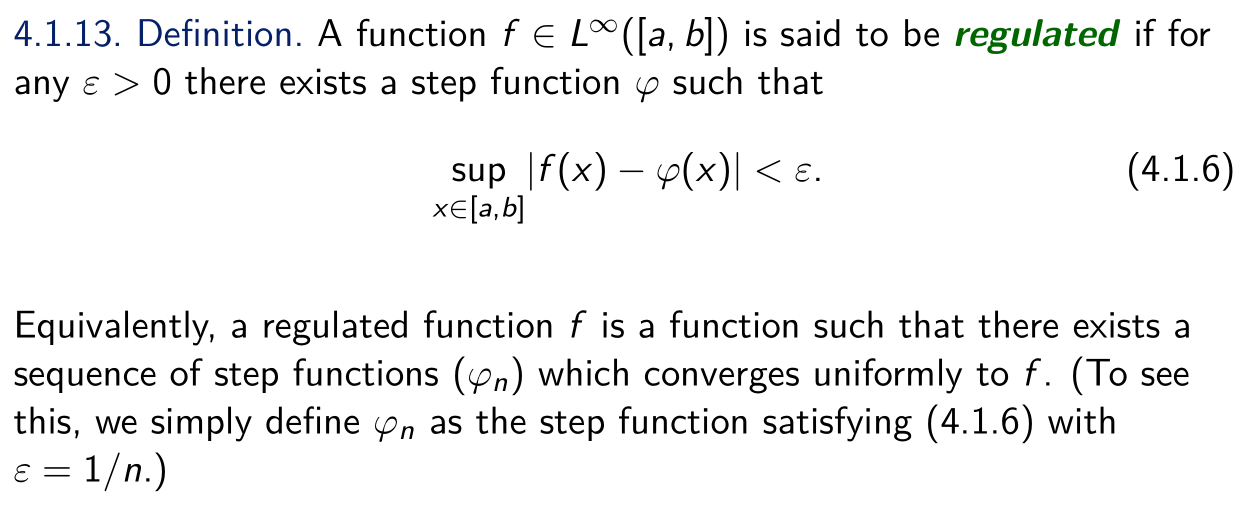
\includegraphics[width=0.9\textwidth]{2020-12-02-11-57-35.png}
    \end{figure}

    \textbf{Remark:}
    \begin{itemize}
        \item The \textit{equivalent description} of 4.1.13. Definition is more intuitive: We seek for a sequence of step functions that converge \textbf{uniformly} to the target function.
        \item The continous a.e.\footnote[frame]{``a.e.'' is the abbreviate of ``almost everywhere''.} functions on a closed interval are regulated. i.e. $\mathrm{PC}([a,b])\subset\mathrm{Reg}([a,b])$
    \end{itemize}

\end{frame}

\begin{frame}
    \frametitle{Regulated Integral}
    \begin{figure}[H]
        \centering
        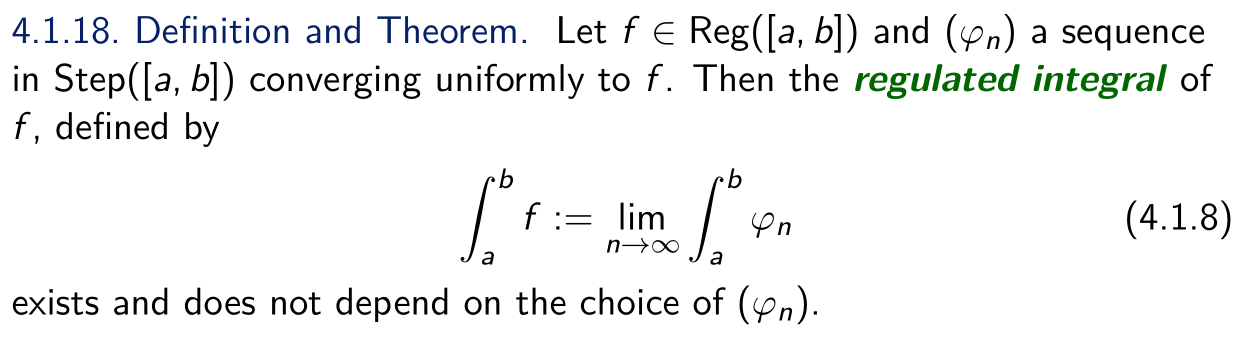
\includegraphics[width=0.9\textwidth]{2020-12-02-12-08-32.png}
    \end{figure}
    \begin{figure}[H]
        \centering
        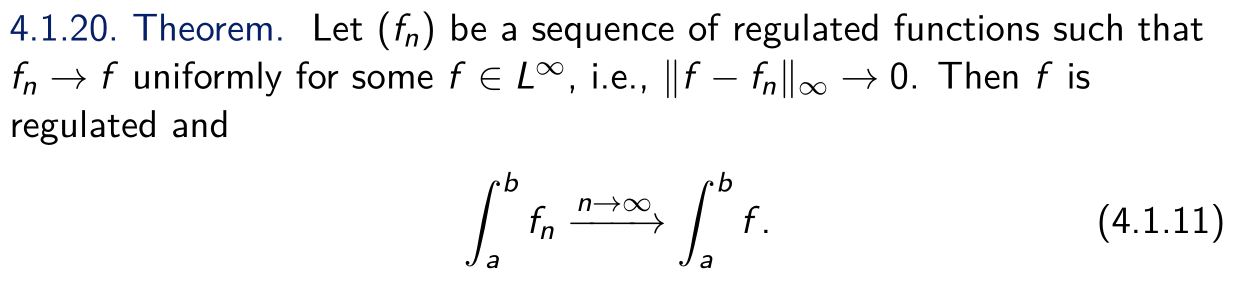
\includegraphics[width=0.9\textwidth]{2020-12-02-12-09-22.png}
    \end{figure}
\end{frame}

\begin{frame}
    \frametitle{Exercise}
    Consider the function
    \begin{figure}[H]
        \centering
        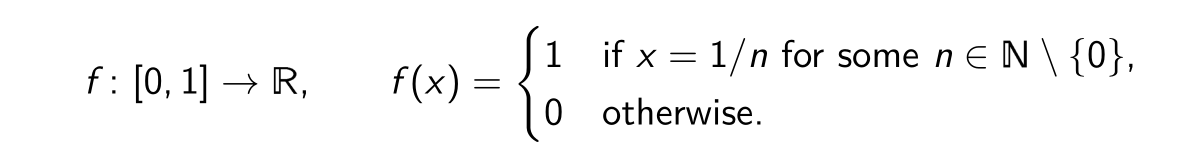
\includegraphics[width=0.9\textwidth]{2020-12-02-12-24-56.png}
    \end{figure}
    Is the function regulated?
\end{frame}

\begin{frame}
    \frametitle{Exercise}
    True or False?
    \begin{enumerate}
        \item $f(x)=x^3+e^x$ on $[-1,1]$ is regulated.
        \item
              Since $f(x)=x^{2}$ is regulated on each $[-n, n],$ where $n \in \mathbb{N}, f$ is regulated on $\mathbb{R}$
              because we can let $n \rightarrow \infty$
        \item A continuous function is piecewise continuous
        \item Let $f,$ g be two real-valued function defined on $[0,1] .$ Furthermore, assume $f-g=x,$ then the equation $\int_{0}^{1}(f-g)=\int_{0}^{1} f-\int_{0}^{1} g=\frac{1}{2}$ holds.
        \item Let $f \in \operatorname{Reg}([0,1]),$ let $g$ be a real-valued function. Then $f \circ g$ is regulated.
    \end{enumerate}
\end{frame}

\subsection{Darboux Integral}
\begin{frame}
    \frametitle{Darboux Integral}
    \begin{figure}[H]
        \centering
        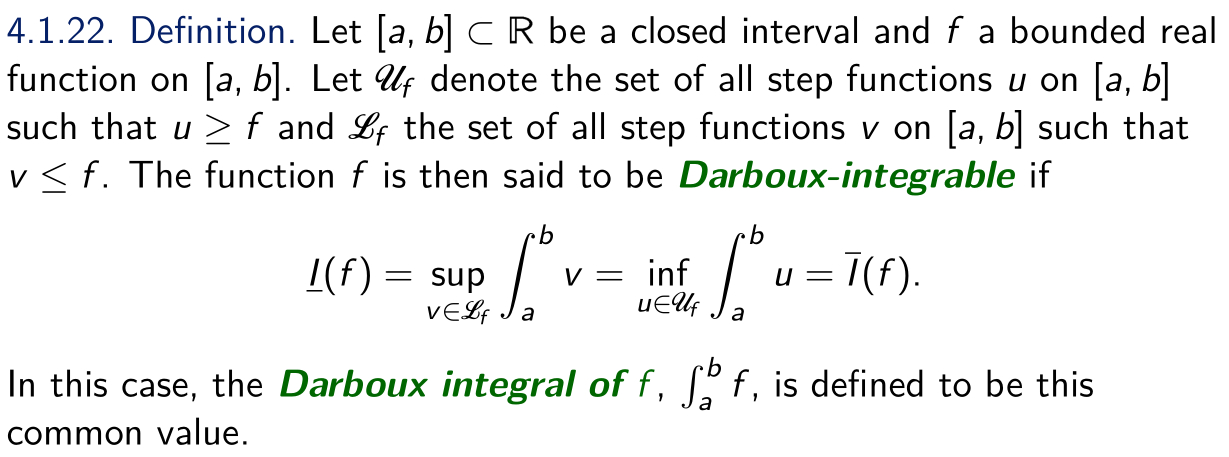
\includegraphics[width=0.9\textwidth]{2020-12-02-12-11-33.png}
    \end{figure}
    \textbf{Question: }True or false?\\
    If $\int_a^b|f|$ is Darboux integrable, $\int_a^b f$ is Darboux integrable.
\end{frame}

\begin{frame}
    \frametitle{Exercise}
    Consider the function
    \begin{figure}[H]
        \centering
        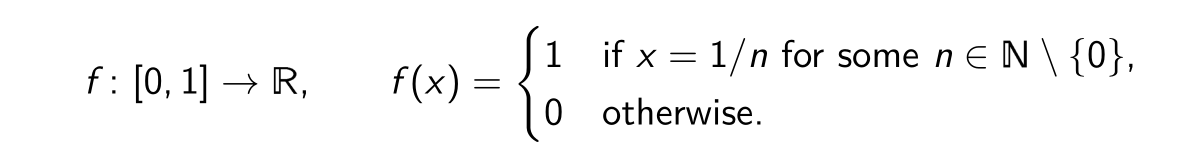
\includegraphics[width=0.9\textwidth]{2020-12-02-12-24-56.png}
    \end{figure}
    Is the function Darboux integrable?
\end{frame}

\subsection{Riemann Integral}
\begin{frame}
    \frametitle{Riemann Integral}
    \begin{figure}[H]
        \centering
        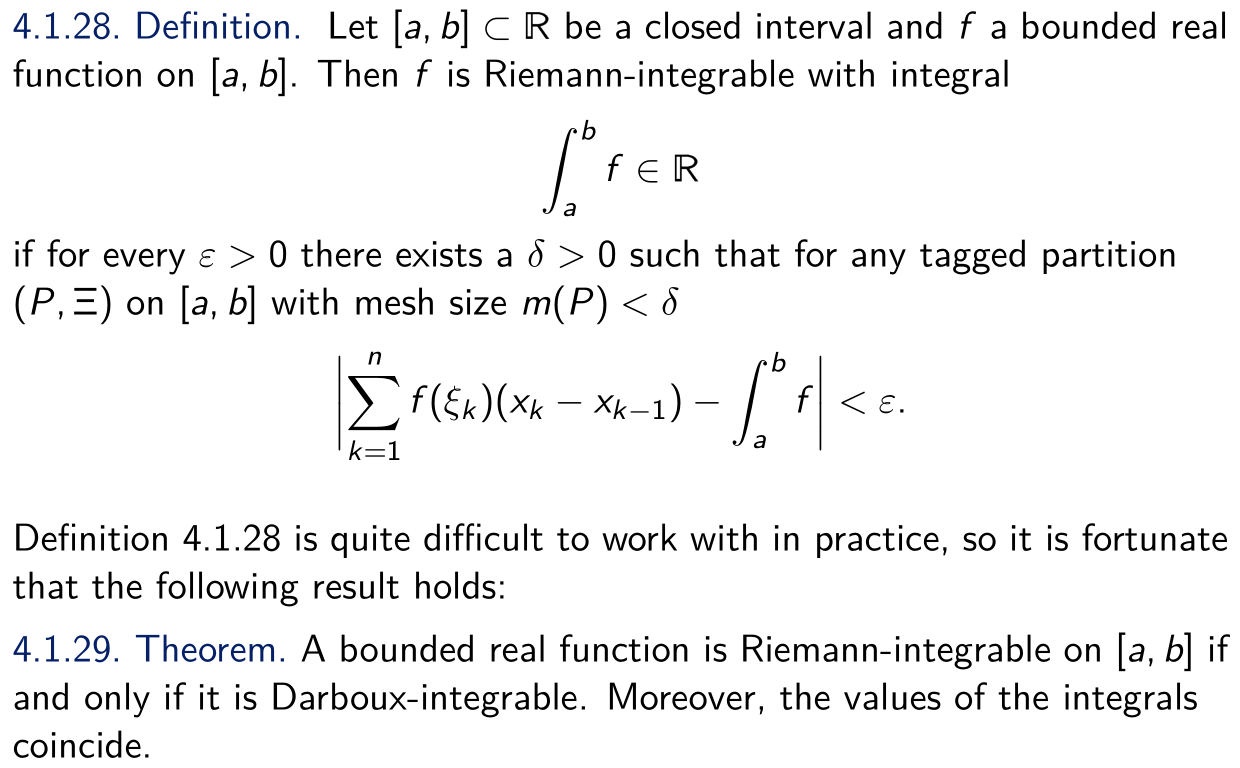
\includegraphics[width=0.9\textwidth]{2020-12-02-12-12-35.png}
    \end{figure}
\end{frame}

\begin{frame}
    \frametitle{Darboux Integral vs. Riemann Integral}
    Describe in words the difference between \textbf{Darboux Integral} and \textbf{Riemann Integral}. How are these two concepts different? If you can, state some properties that they have in common or that serve to differentiate them from each other. Is one of them also always an example of the other? Give examples.
    \nullspace
    This exercise is left for you!
\end{frame}

\section{Integration in Practice}
\subsection{The Fundamental Theorem of Calculus}
\begin{frame}
    \frametitle{The Fundamental Theorem of Calculus}
    \begin{figure}[H]
        \centering
        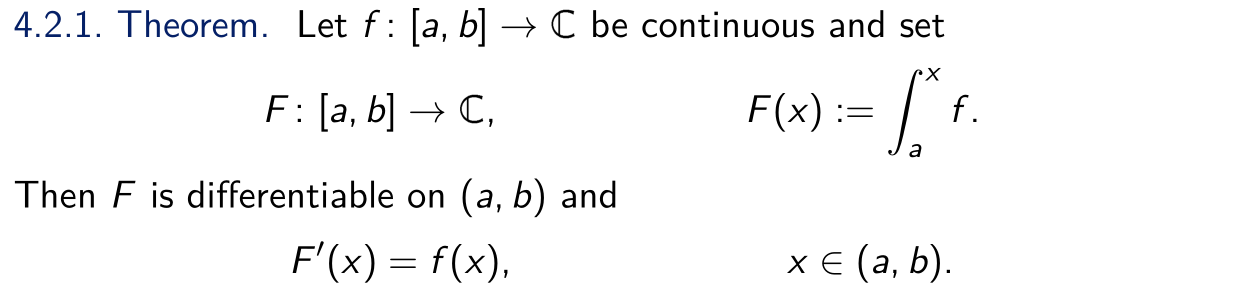
\includegraphics[width=0.9\textwidth]{2020-12-02-13-38-29.png}
    \end{figure}
\end{frame}

\begin{frame}
    \frametitle{The Fundamental Theorem of Calculus}

    \begin{figure}[H]
        \centering
        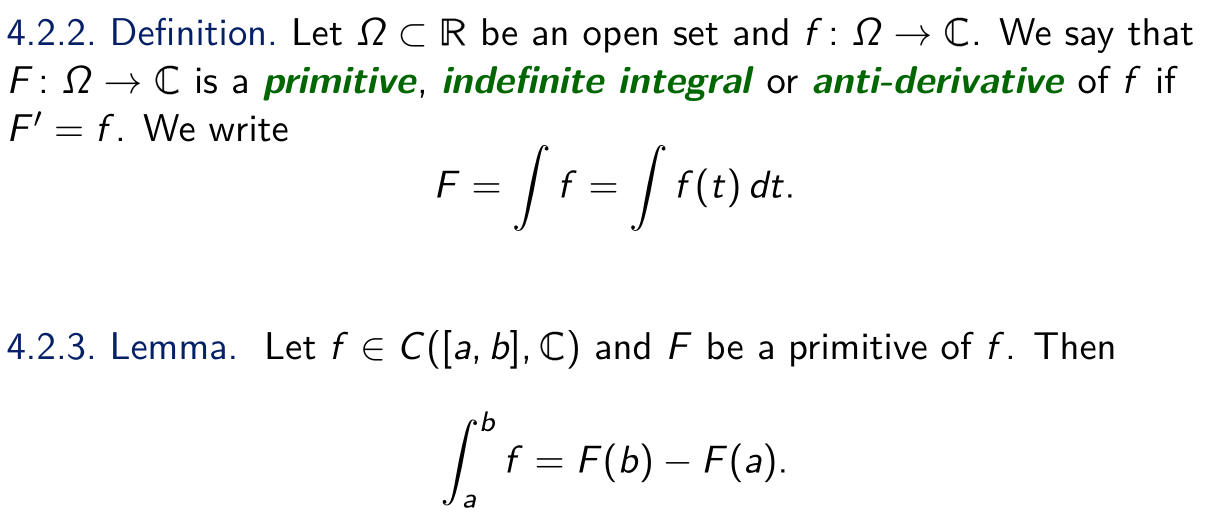
\includegraphics[width=0.9\textwidth]{2020-12-02-13-39-39.png}
    \end{figure}

    \textbf{Remark:} This result shows that we can regard integration as ``inverse differentiation''. We can then calculate various integrals simply by guessing their primitives.\\
    \textbf{Question:} Since $\int_{-1}^{1} \frac{1}{x^{2}+1}=\left.\arctan x\right|_{-1} ^{1}=\frac{\pi}{2}$ but $\int_{-1}^{1} \frac{1}{x^{2}+1}=-\left.\arctan \frac{1}{x}\right|_{-1} ^{1}=$
    $-\frac{\pi}{2}$. Where is wrong?
\end{frame}

\begin{frame}
    \frametitle{Exercise}

    Calculate the derivative of $g:[a,b]\to\R,$ $$g(x)=\int_{p(x)}^{q(x)}f,$$ where $f,p,q$ are differentiable on $(a,b)$.

\end{frame}


\subsection{Substitution Rule}
\begin{frame}
    \frametitle{Substitution Rule}

    \begin{figure}[H]
        \centering
        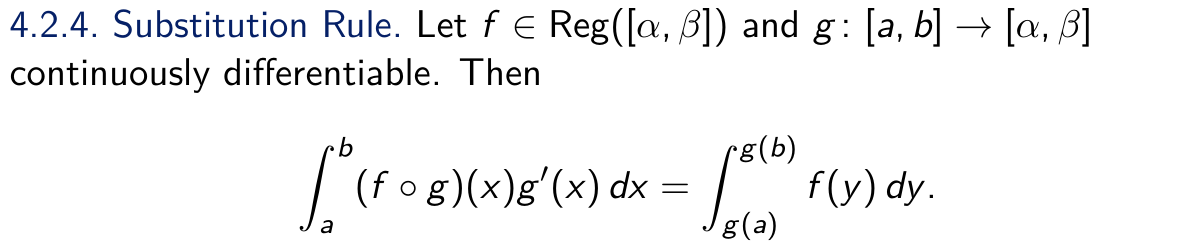
\includegraphics[width=0.9\textwidth]{2020-12-02-13-41-48.png}
    \end{figure}
    \begin{figure}[H]
        \centering
        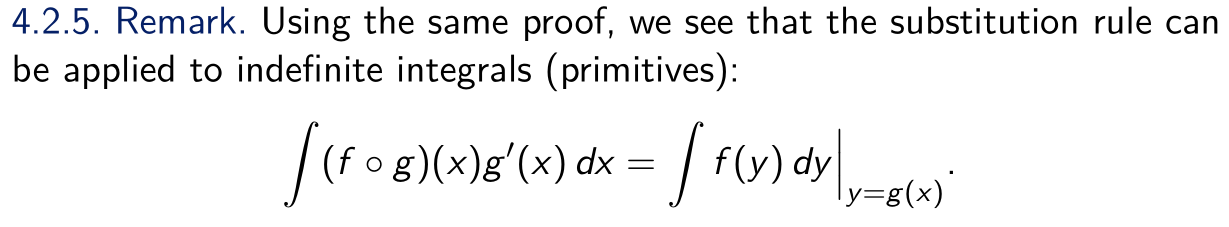
\includegraphics[width=0.9\textwidth]{2020-12-02-13-42-07.png}
    \end{figure}
    \textbf{Remark:} We can, to some extent, abuse the Leibniz notation to memorize substitution rule. You are free to use it in the exam.

\end{frame}
\begin{frame}
    \frametitle{Exercise}
    Let $f,g\in C([-a,a])$ such that $g$ is even function and $f(x)+f(-x)=A$. Prove $$\int_{-a}^a fg=A\int_0^a g.$$
    \nullspace Calculate
    $$\int\dfrac{x}{3x^2+6x+10}$$
    Calculate
    $$\int\dfrac{1}{\sin(x)\cos^3(x)}$$
\end{frame}

\subsection{Integration by Parts}
\begin{frame}
    \frametitle{Integration by Parts}
    \begin{figure}[H]
        \centering
        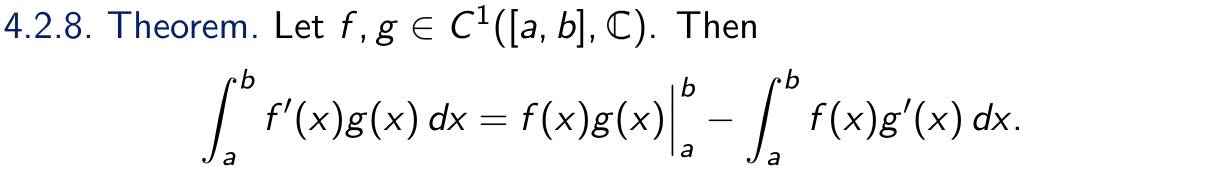
\includegraphics[width=0.9\textwidth]{2020-12-02-13-43-47.png}
    \end{figure}
\end{frame}

\begin{frame}
    \frametitle{Exercise}
    Calculate
    $$\int\left(3 t+t^{2}\right) \sin (2 t) d t$$

\end{frame}

\subsection{Improper Integrals}
\begin{frame}
    \frametitle{Improper Integrals}

    \begin{figure}[H]
        \centering
        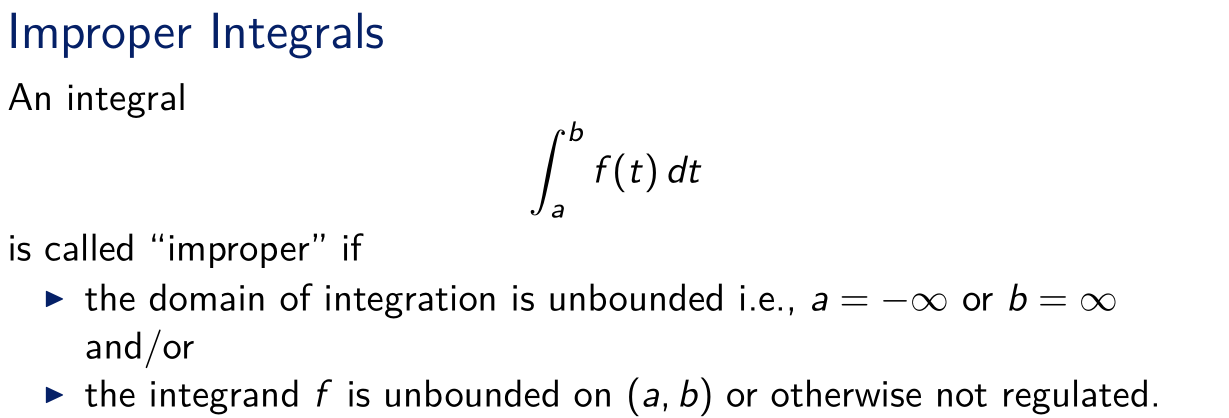
\includegraphics[width=0.9\textwidth]{2020-12-02-13-50-24.png}
    \end{figure}

    \textbf{Remark:} See detailed definitions on Slides 562. We well defined it using limit.
\end{frame}

\begin{frame}
    \frametitle{Exercise}

    Determine if the following integral converges or diverges. If the integral converges determine its value.
    $$\int_{0}^{4} \frac{x}{x^{2}-9} d x$$
    $$\int_{-\infty}^{0} \frac{e^{\frac{1}{x}}}{x^{2}} d x$$

\end{frame}

\begin{frame}
    \frametitle{Cauchy Criterion for Functions}
    \begin{figure}[H]
        \centering
        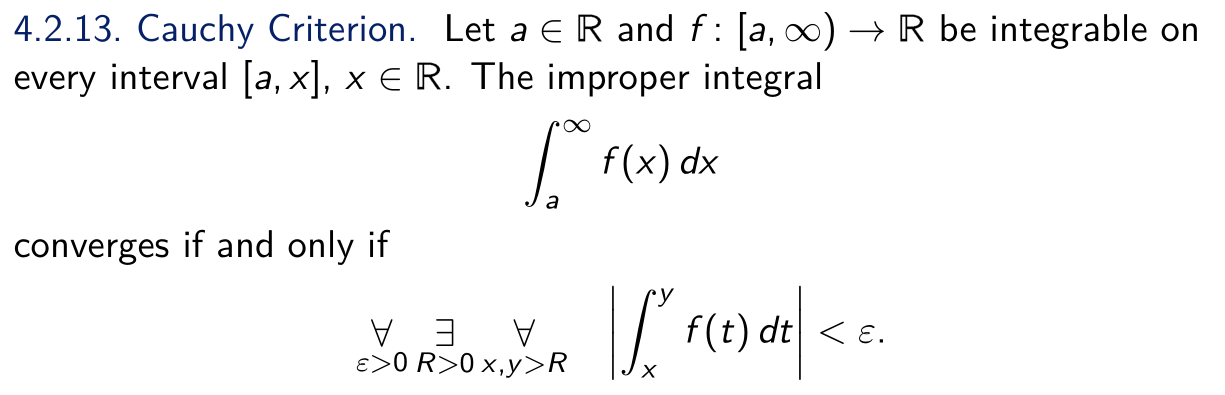
\includegraphics[width=0.9\textwidth]{2020-12-02-13-52-20.png}
    \end{figure}
\end{frame}

\begin{frame}
    \frametitle{Results}
    \begin{itemize}
        \item 4.2.16. Comparison Test.
        \item 4.3.1. Integral Test.
    \end{itemize}
\end{frame}

\begin{frame}
    \frametitle{Exercise}

    Use the Comparison Test to determine if the following integral converges or diverges.
    $$\int_{1}^{\infty} \frac{z-1}{z^{4}+2 z^{2}} d z$$

\end{frame}

\section{Application of Integration}
\subsection{Taylor's Theorem}
\begin{frame}
    \frametitle{Taylor's Theorem}

    \begin{figure}[H]
        \centering
        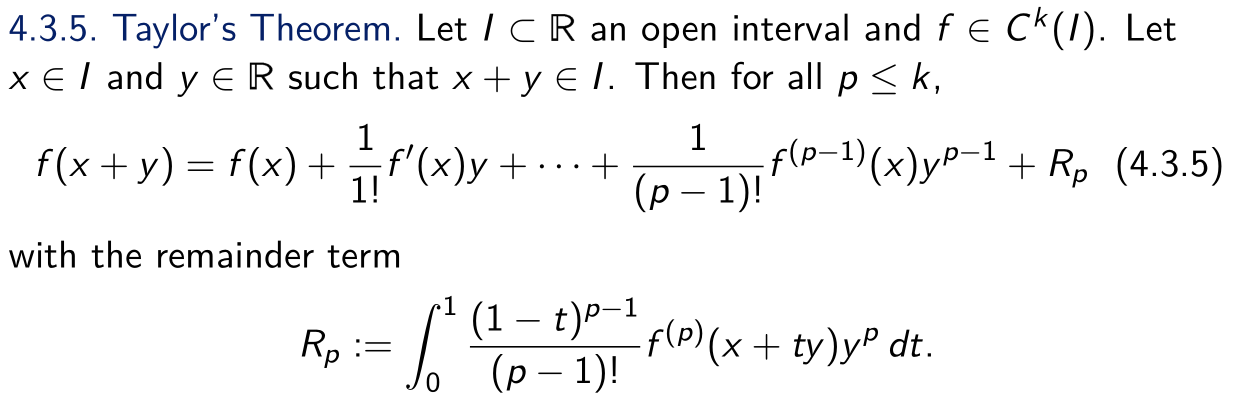
\includegraphics[width=0.9\textwidth]{2020-12-02-13-55-33.png}
    \end{figure}
    \textbf{Remark:} Memorize the remainder term. (so-called Lagrange form)
\end{frame}

\begin{frame}
    \frametitle{Taylor Series And Analyticity}

    \begin{figure}[H]
        \centering
        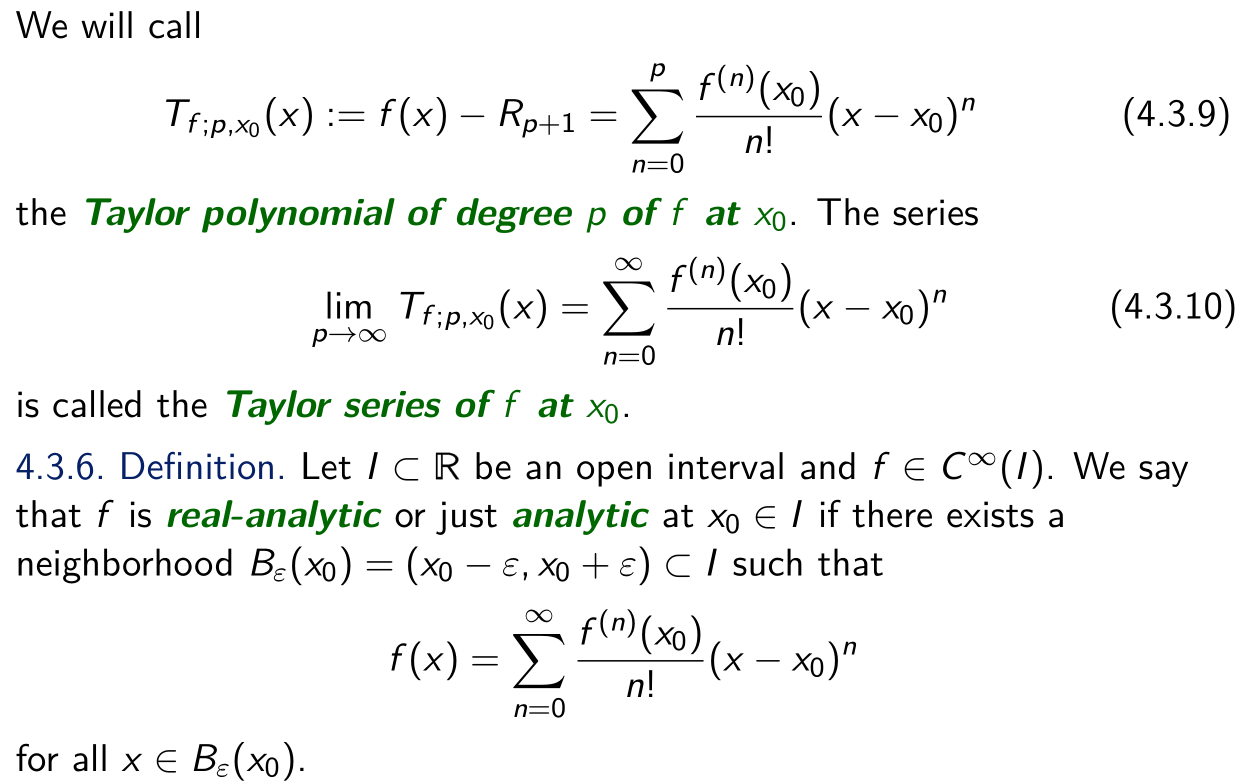
\includegraphics[width=0.9\textwidth]{2020-12-02-13-59-15.png}
    \end{figure}

\end{frame}

\begin{frame}
    \frametitle{Remarks}

    \begin{itemize}
        \item \emph{Taylor's series} is extremely useful in engineering fields because it offers a fine approximation of the function's behavior near some point. For example, oscillation analysis.
        \item However, in reality, since that we can only use polynomials of finite degrees, the taylor expansion degenerates rapidly when approaching to the radius of convergence.
        \item Some functions are not analytic. i.e. cannot be approximated by Taylor's theorem. But these weird functions never appear in engineering applications.
    \end{itemize}

\end{frame}

\section{Extension}
\subsection{Euler Gamma Function}
\begin{frame}
    \frametitle{Euler Gamma Function}
    \begin{figure}[H]
        \centering
        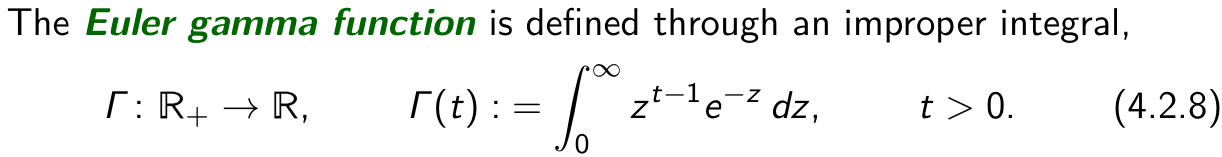
\includegraphics[width=0.9\textwidth]{2020-12-02-14-11-31.png}
    \end{figure}
    Euler Gamma Function is the unique \emph{analytic continuation} of factorial function $(\cdot - 1)!$. It is log-convex on $\R^+$ (increases faster than exponential function). Moreover, it is differentiable.
    \begin{columns}
        \begin{column}{0.5\textwidth}
            \begin{figure}[H]
                \centering
                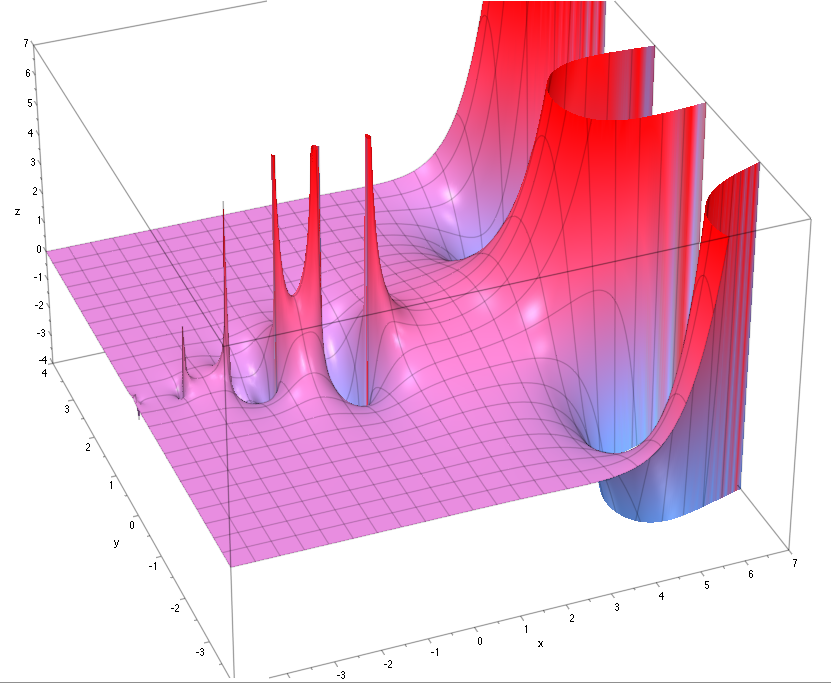
\includegraphics[width=0.7\textwidth]{2020-12-02-14-15-47.png}
                \caption{Real Part Plot}
            \end{figure}
        \end{column}
        \begin{column}{0.5\textwidth}
            \begin{figure}[H]
                \centering
                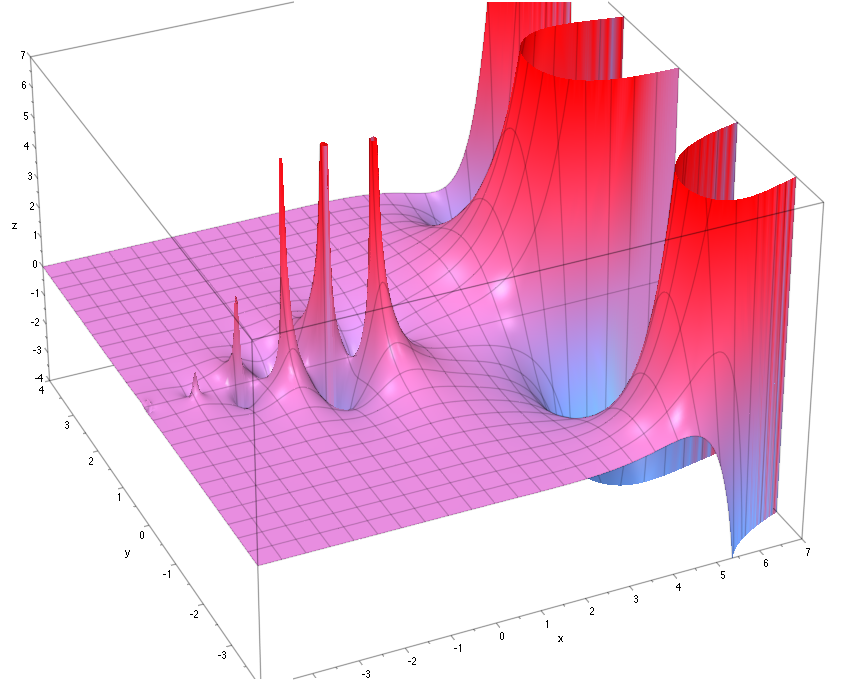
\includegraphics[width=0.7\textwidth]{2020-12-02-14-16-12.png}
                \caption{Imaginary Part Plot}
            \end{figure}
        \end{column}
    \end{columns}
\end{frame}
\subsection{Riemann Zeta Function}
\begin{frame}
    \frametitle{Riemann Zeta Function}
    \begin{figure}[H]
        \centering
        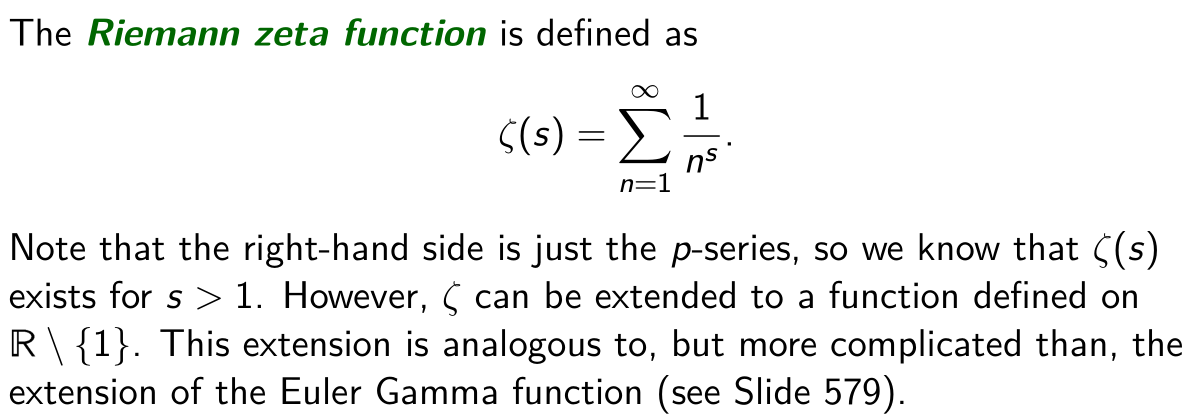
\includegraphics[width=0.9\textwidth]{2020-12-02-14-29-10.png}
    \end{figure}

    \begin{figure}[H]
        \centering
        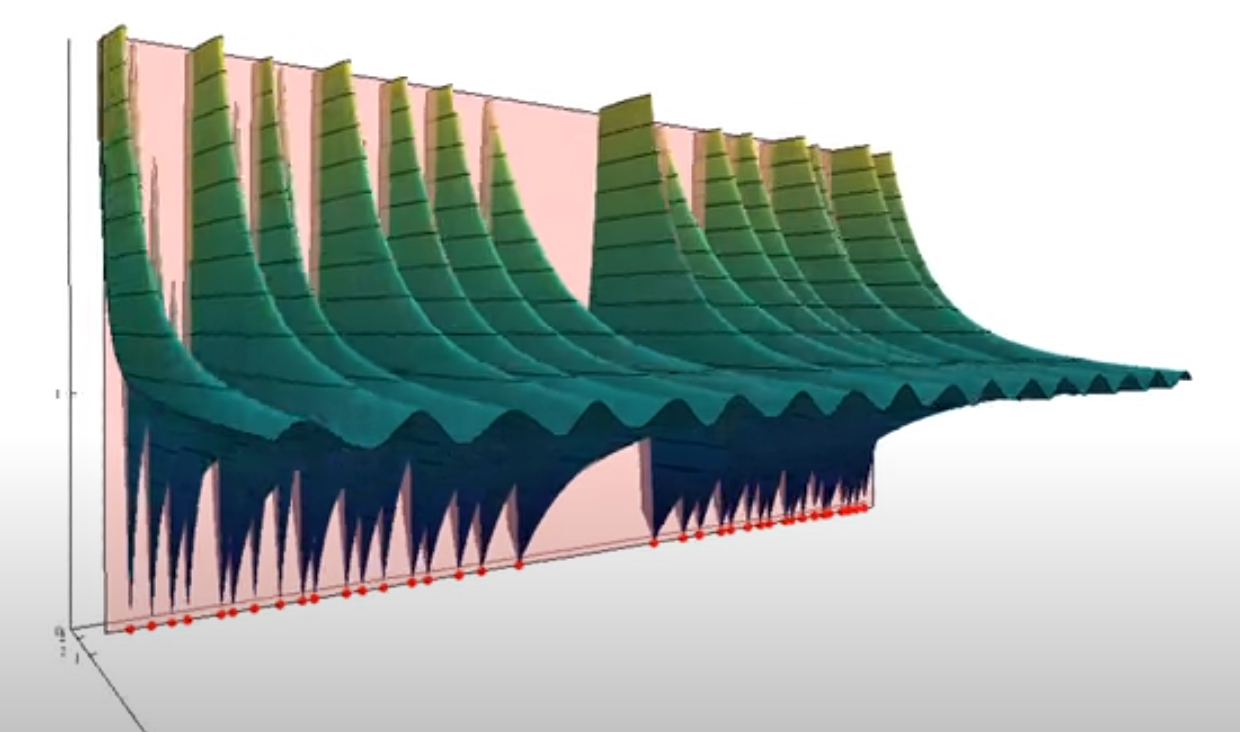
\includegraphics[width=0.5\textwidth]{2020-12-02-14-28-34.png}
    \end{figure}
\end{frame}
\begin{frame}
    \frametitle{Riemann Zeta Function}

    Here is a very good video in simple terms illustrating the Riemann Zeta functions, as well as the famous \emph{Riemann Hypothesis}:
    \begin{center}
        \begin{figure}[H]
            \centering
            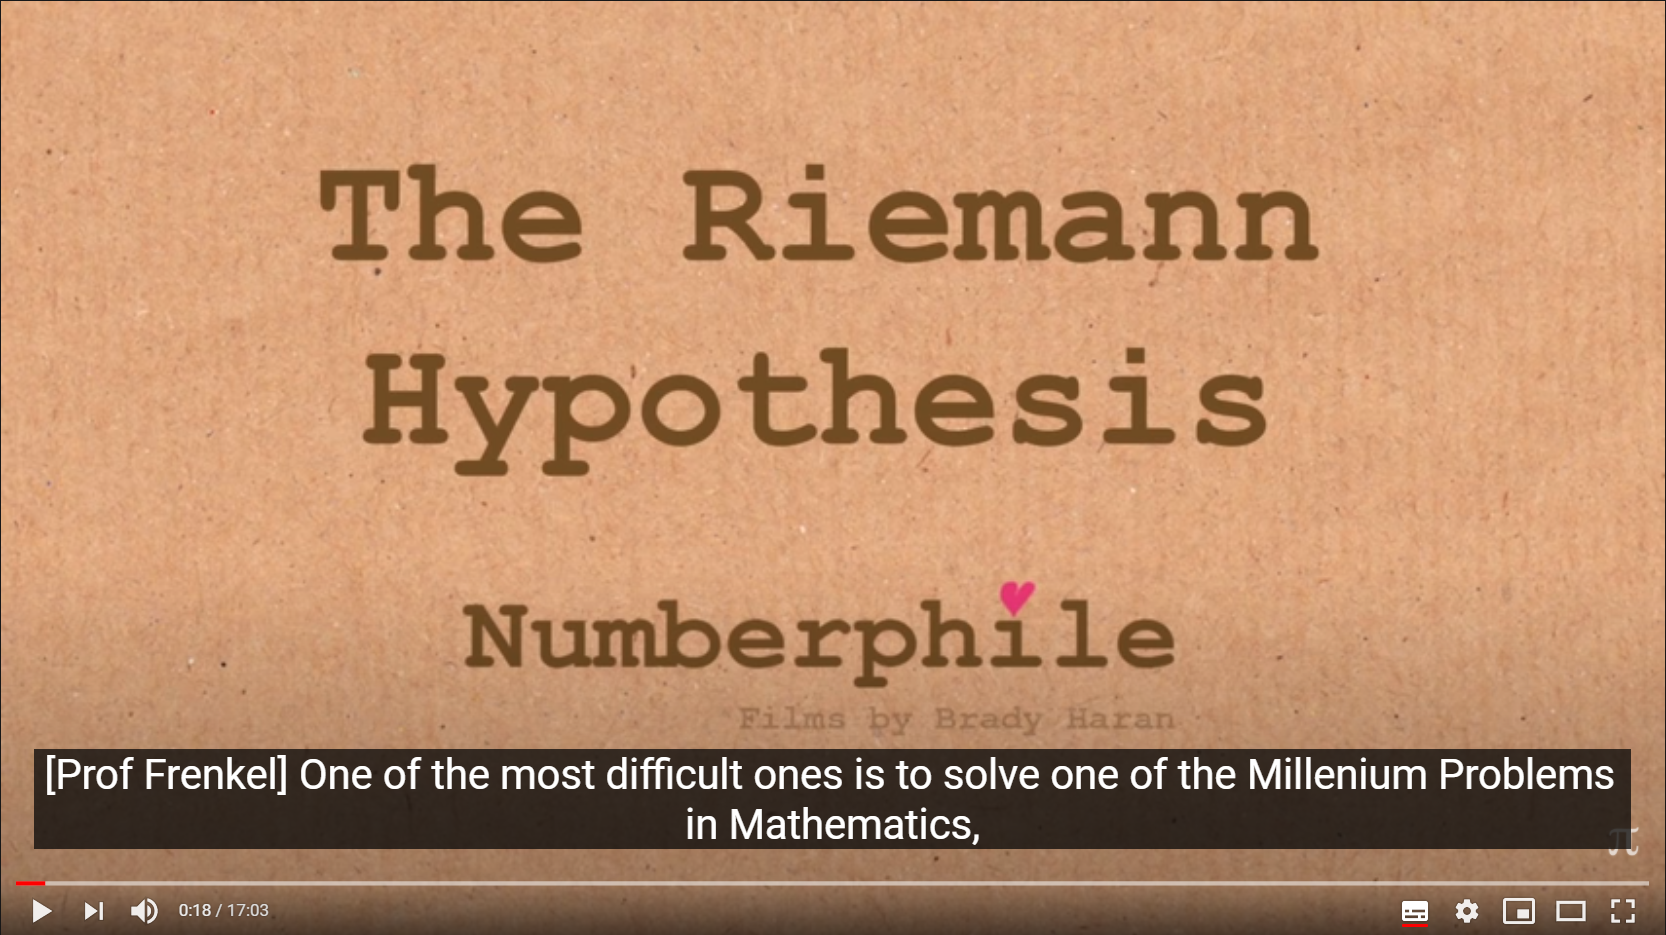
\includegraphics[width=0.8\textwidth]{2020-12-02-14-48-15.png}
        \end{figure}
        \href{https://www.youtube.com/watch?v=d6c6uIyieoo}{[Link] \textit{Riemann Hypothesis - Numberphile}}
    \end{center}
    Go to watch that when you are free!

\end{frame}
\begin{frame}
    \frametitle{Abel Sum}

    \begin{figure}[H]
        \centering
        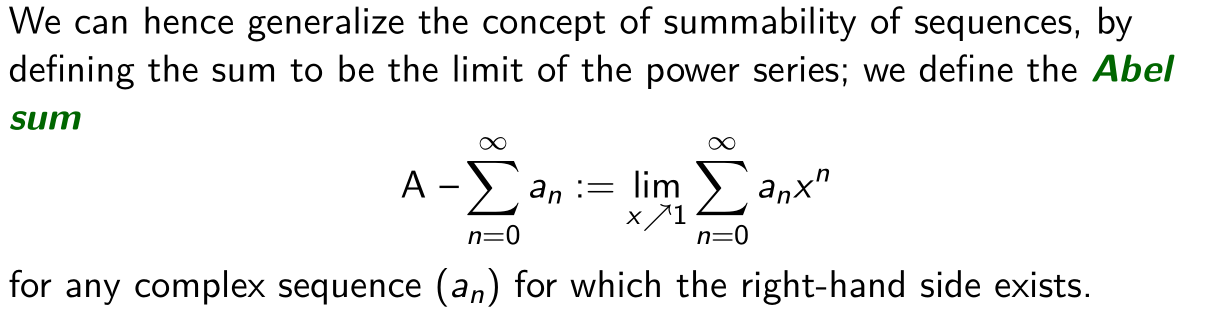
\includegraphics[width=0.9\textwidth]{2020-12-02-14-30-21.png}
    \end{figure}

\end{frame}

\begin{frame}
    \frametitle{Tips}
    \begin{itemize}
        \item Practice makes perfect. Here is a website with lots of typical integral problems as well as detailed solutions. You can pick up some as exercises if you want. \href{https://tutorial.math.lamar.edu/Problems/CalcII/IntTechIntro.aspx}{Paul's Online Notes}
        \item Having taken two vv186 exams, (I believe) you have enough experience and confidence to take the final. The final exam is similar to the two midterm exams in term of duration, compositions.
        \item You have made your first step into the fascinating and beautiful math world. Congratulations! Helping you guys see the wonderfulness of math is my motivation to be a TA, and I am happy to realize that many of you start to do so rather than bearing its tediousness. I appreciate all of your hard work in this tough semester, and am honored to being your TA. Wish you enjoy this journey and have a good grade!
    \end{itemize}
\end{frame}

\begin{frame}
    \frametitle{Not End}
    \vspace{1cm}
    \begin{center}
        \Huge
        Forever\\
        Have Fun \\
        And \\
        Learn Well!\footnote[frame]{Special acknowledgement to former TA \textbf{Zhang Leyang}, who offered plenty of exercises and advice to my recitation class.}
    \end{center}
\end{frame}

\end{document}